\section{Suggestions for improvement}\label{jiveSuggestions}

While exploring the features of JIVE, a few issues regarding use and behavior were encountered.
None of these issues can be considered to be major, but they still expose a potential for improvement.
This section will point out some of the issues, and provide suggestions on what can be done to improve them.
~\\

\subsection{Visual changes to the diagrams}\label{jiveSuggestionsVisual}
%oppdage indre typer
In both diagrams, object instances are labeled with the name of the object type, and an instance-number, separated with a colon, e.g. `PersonPanel:1'.
While this provides the expected information, it is affected by the way Java handles the naming of anonymous inner types -- classes that are defined within another class, and not given a name by the developer.
Java automatically names these classes by appending a dollar sign and a identifying number to the name of the class they are defined within, e.g. `PersonPanel\$1'.
\gls{gui}-programs are written with several such classes to handle user input, each implementing a listener-interface of some kind, and they show up in the diagrams with their generated names, that do not reflect the purpose of the class.
The ability to detect an inner type with a generic name, and display the interface it implements, instead of is actual name should help with this issue.
Among others, listener-heavy programs should become more understandable, as the kind of listeners in use will be clearly visible, removing the need to guess based on when they are invoked in the sequence-diagram.
\autoref{fig:contOving4Changes} illustrates this as the change from part a to part b.
~\\

%koble listeners til det de lytter på
To further help users identify listeners, they could be visually linked to the objects they are listening to in the contour-diagram, making it clearly visible which object is being listened to by the different listeners, as illustrated in part c of \autoref{fig:contOving4Changes} illustrates this change, along with the relabeled objects.
While the effect is possible to achieve by applying an appropriate filter, this filter must let a large amount of objects through, causing the diagrams to become cluttered and challenging to navigate.
On the other hand, the effect of the listener being triggered is clearly visible in the sequence diagram, and it is possible that this is easy enough to connect with a users interactions with a program, so that such a link will not be necessary.
~\\

%visualisere mvc-komonenter
A last visual change would be to attempt further identification of the components that make up an \gls{mvc}-architecture, and highlight them.
Being a change focusing solely on a specific architecture, it has to be possible to deactivate when not needed.
The challenge with this feature is to find a way to identify the different components.
While listeners can usually be identified by their name, of by their implementation of certain interfaces, this is not necessarily the case for models and controllers.
Another challenge is to not add so many new elements to the diagrams that they become chaotic and difficult to read.

Finding ways to highlight the different parts of e.g. an MVC-architecture, making it clearly visible which objects make out the models, views and controllers, may further help the understanding of a program.
But such highlighting must be balanced in order to not create a visual chaos of different colors.
Adding symbols instead of colors might be a better solution, both maintaining the current color-scheme, and adding new information.
The coloring, highlighting and naming of inner types should apply to both of the diagrams.
The biggest challenge with this kind of highlighting, is the process of detection.
While listeners can easily be detected by their implementation of a listener-interface, detecting a controller or a model is not trivial.
One can make assumptions based on class names, but they will be worthless if a program does not match those assumptions, and developers are not likely to change their programs to fit.
~\\

\begin{figure}[H]
	\centering
	\begin{subfigure}{\textwidth}
		\centering
		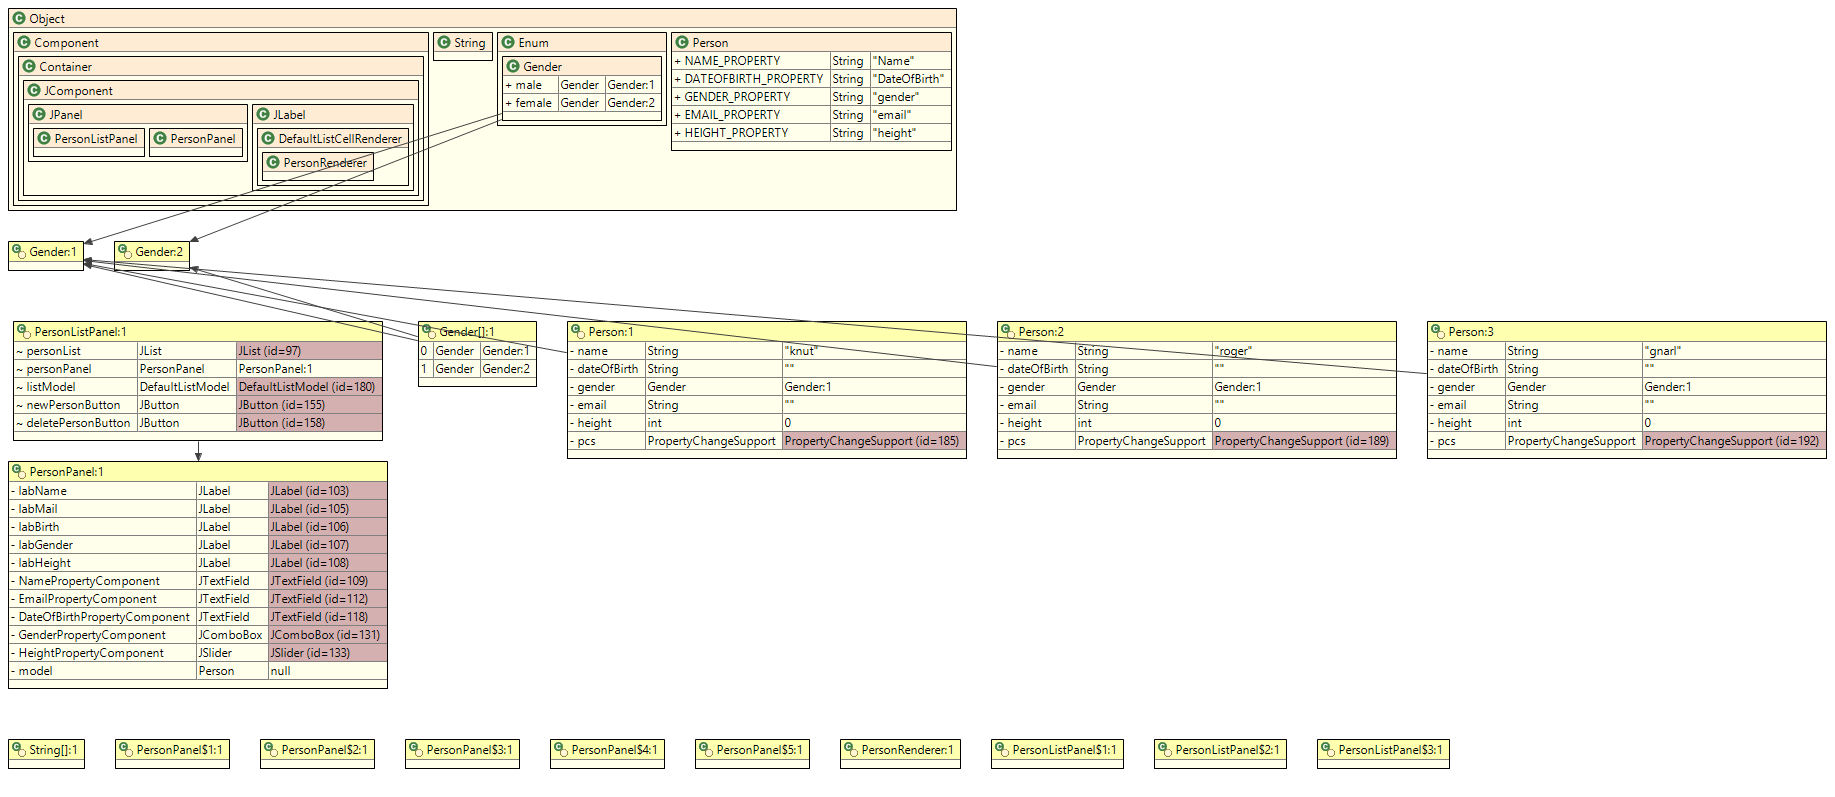
\includegraphics[width=\textwidth, trim= 0 0 0 0, clip]{MMI-Oving4-ObjectDiagInit}
		\caption{Original}
		\label{fig:contOving4ChangesA}
	\end{subfigure}
	\begin{subfigure}{\textwidth}
		\centering
		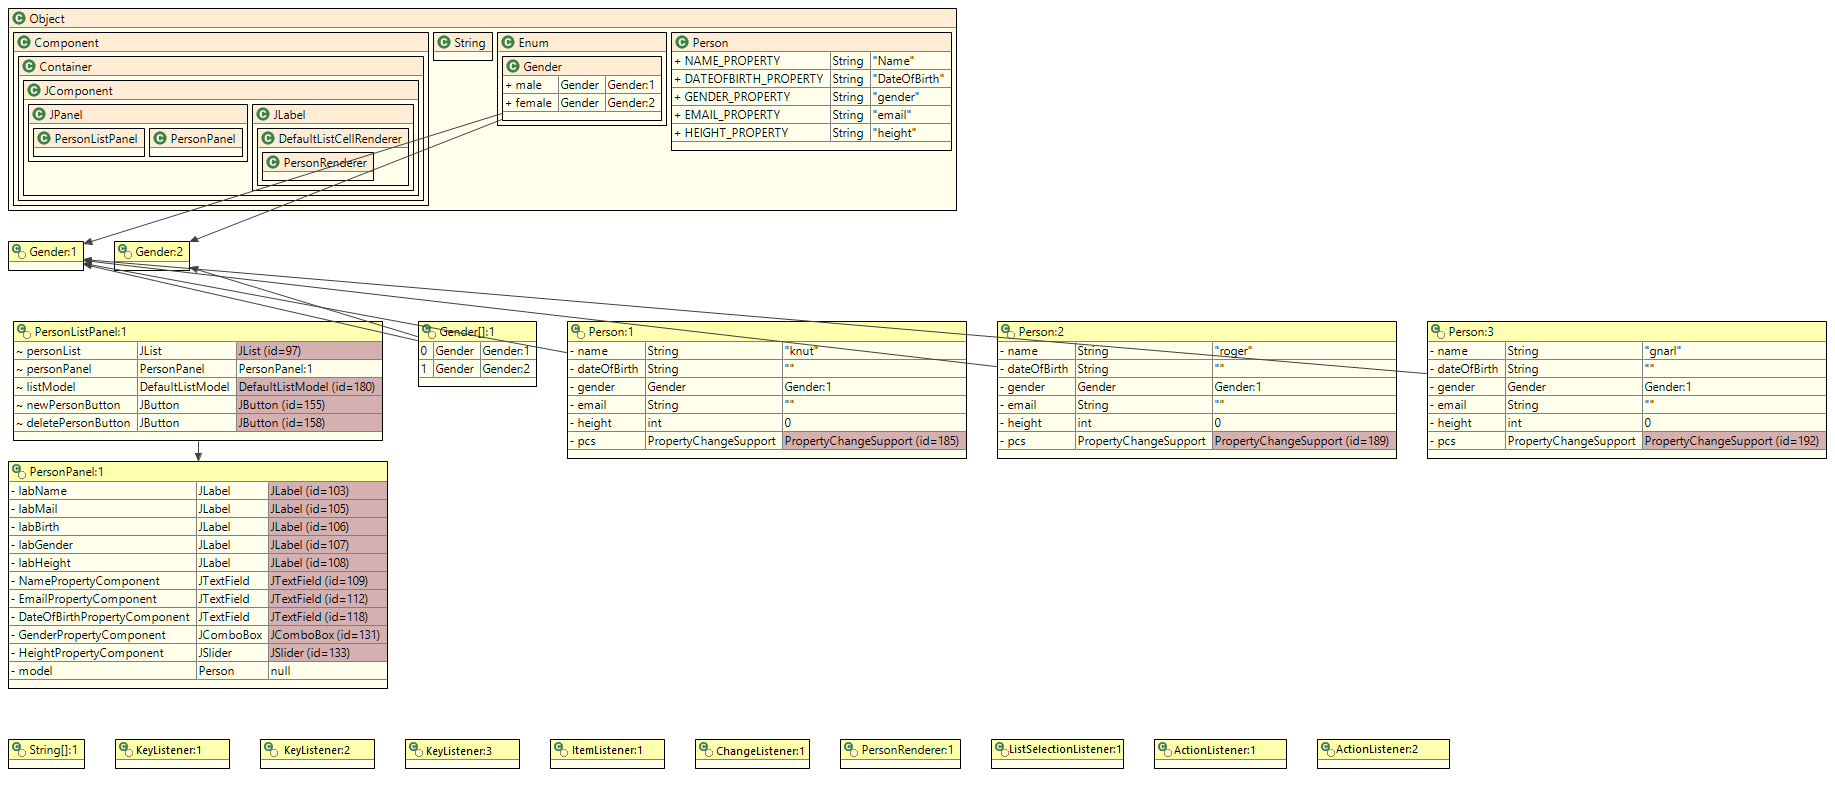
\includegraphics[width=\textwidth, trim= 0 0 0 0, clip]{MMI-Oving4-ObjectDiagInit-edit}
		\caption{Changed naming of inner types}
		\label{fig:contOving4ChangesB}
	\end{subfigure}
	\begin{subfigure}{\textwidth}
		\centering
		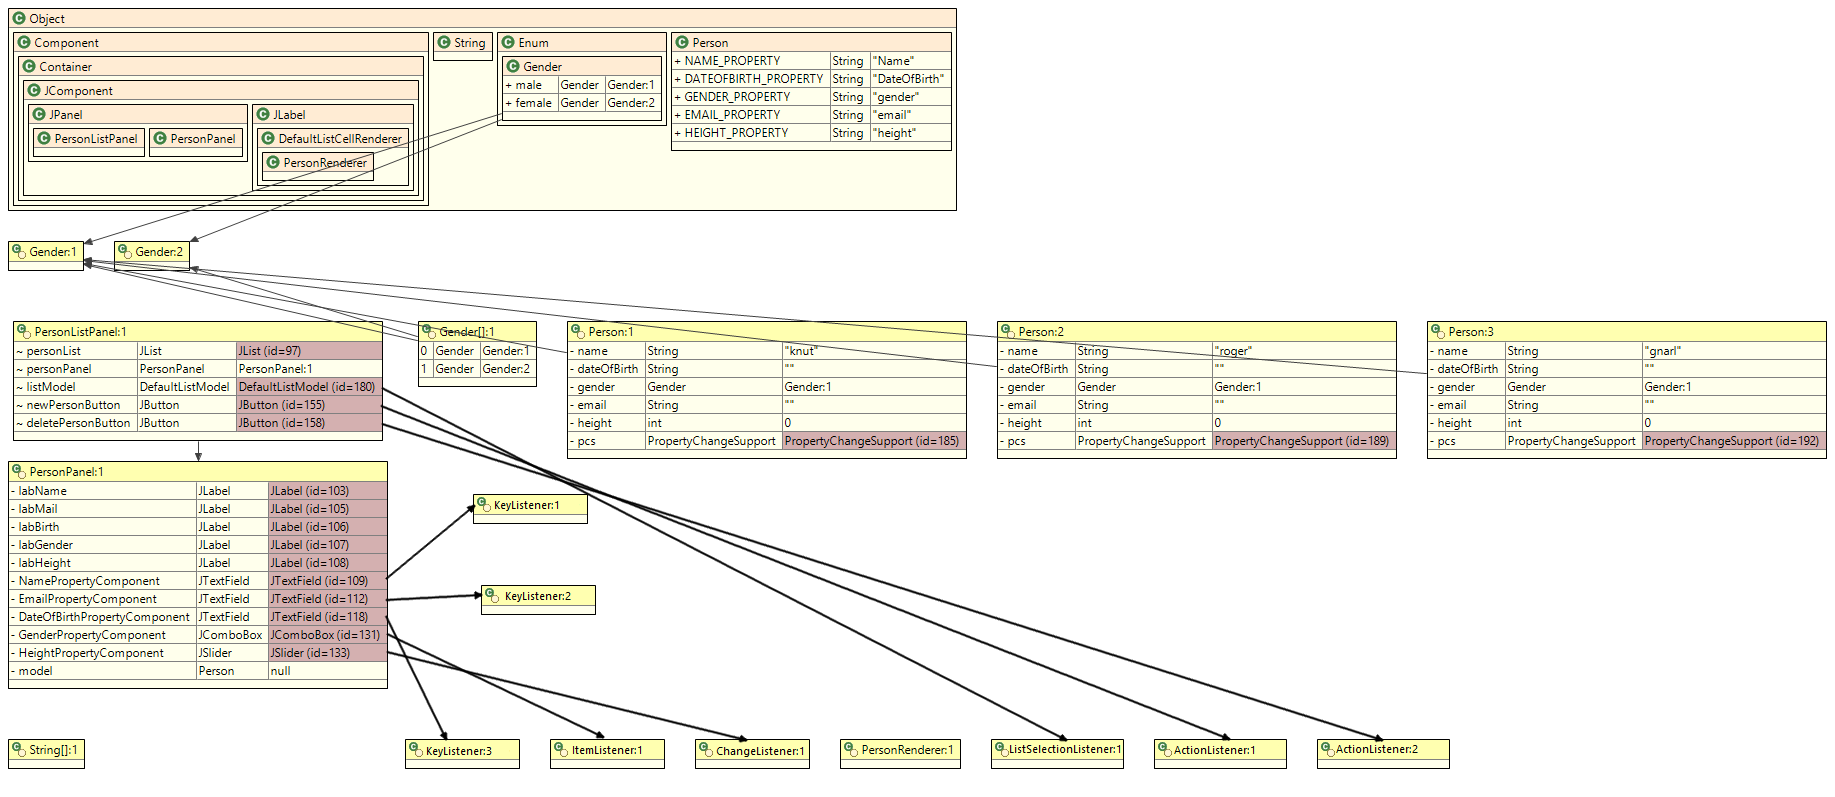
\includegraphics[width=\textwidth, trim= 0 0 0 0, clip]{MMI-Oving4-ObjectDiagInit-edit3}
		\caption{Listeners connected to the object listened to}
		\label{fig:contOving4ChangesC}
	\end{subfigure}
	\caption{Comparison of suggested changes to the contour diagram}
	\label{fig:contOving4Changes} 
\end{figure}
~\\

\subsection{Functional changes}\label{jiveSuggestionsFunctional}
%filter-endringer
Exploring changes to the default exclusion-filter, in order to provide more useful information out of the box, is also an option.
This will provide a better experience for certain scenarios, but may be useless in other cases by providing too much unnecessary information.
A way to easily switch filters by defining presets might be preferable.
The filter might also be extended to support both exclusion and inclusion, allowing a more fine-grained selection of interesting classes.
As an example, one might be interested in ignoring the entire javax-package, but still allowing javax.swing in order to see more \gls{gui}-related objects.
It is also important to not allow too many packages through the filter, as the performance can suffer immensely from logging too many events.
~\\

%bruker-tilpasning av diag
Allowing more ways to interact with the diagrams, e.g. hiding elements or compressing sequences, should improve usability for larger programs and longer runs.
The way the sequence diagrams currently work, object instances are added as they appear, resulting in later method calls to draw lines crossing large parts of the diagram, as shown in \autoref{fig:seqOving4CrossLines}.
~\\

\begin{figure}[H]
	\centering
	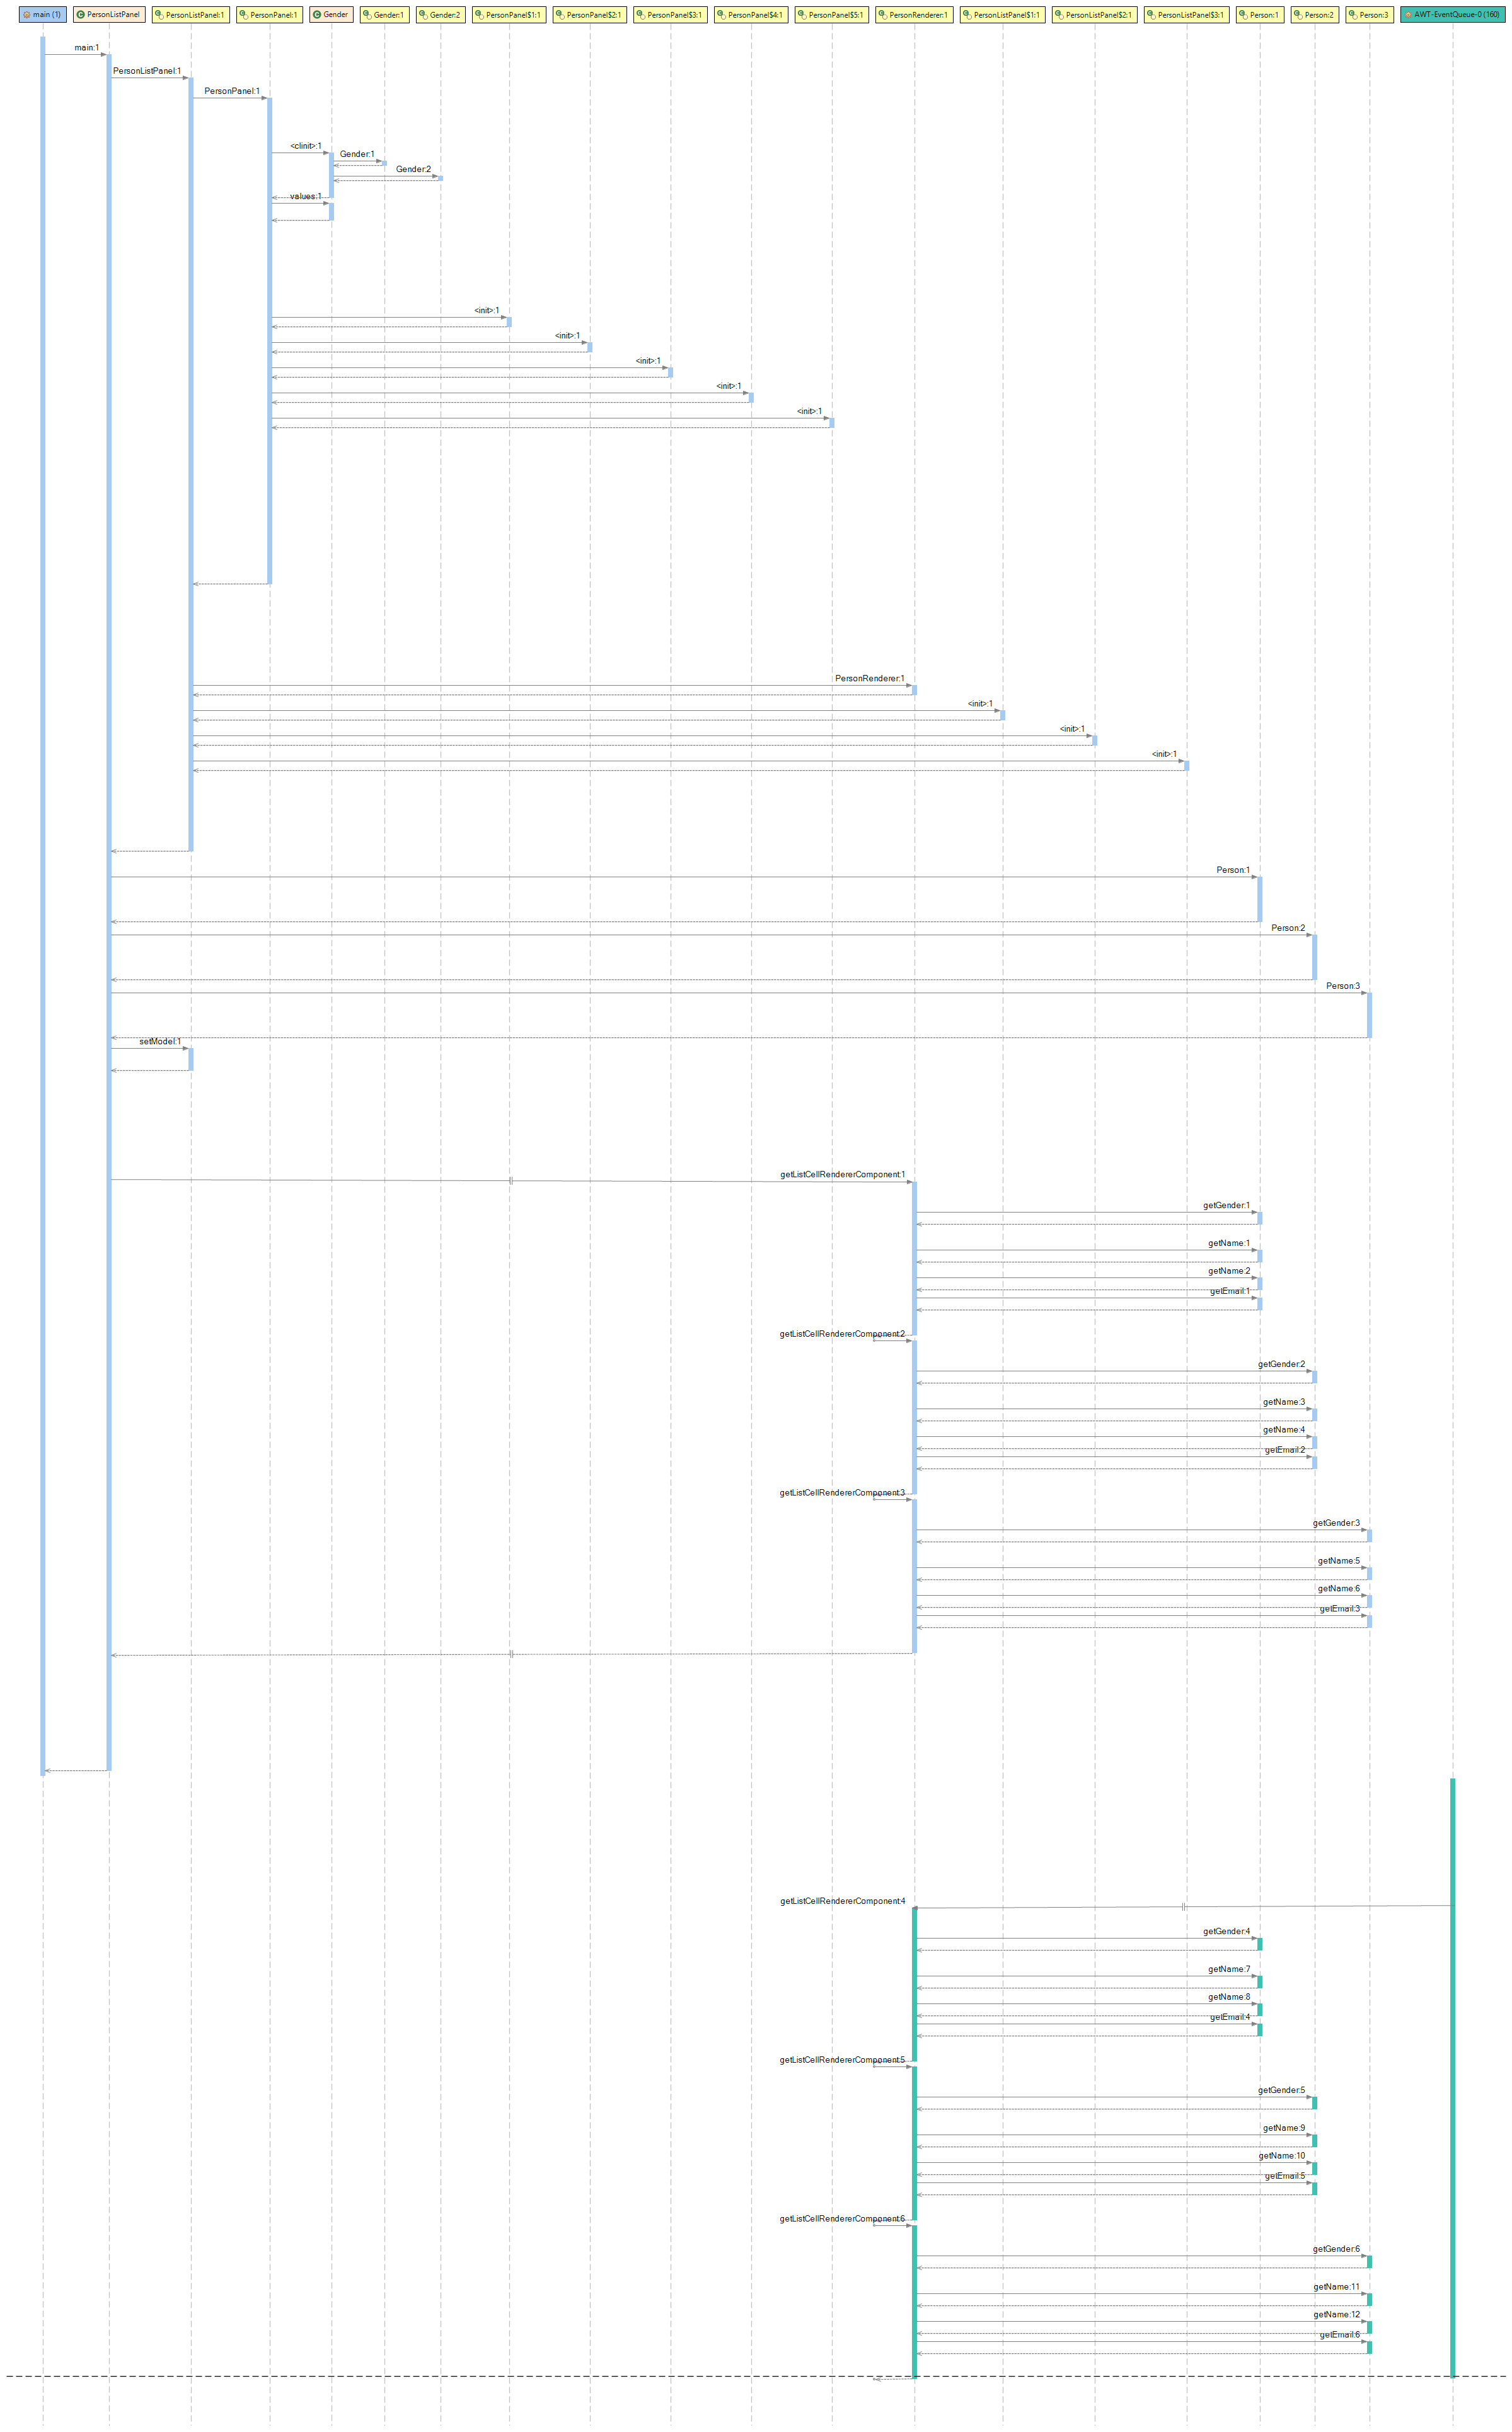
\includegraphics[width=\textwidth, trim= 45cm 7cm 0cm 103cm, clip]{MMI-Oving4-SequenceDiagInit}
	\caption{A section of a larger sequence diagram, showing method calls crossing several unrelated lifelines}
	\label{fig:seqOving4CrossLines}
\end{figure}
~\\

%isolert visning
In the case of exploring events triggered by a listener, the ability to isolate the involved objects, and reorder the diagram could be very useful, providing a clean view of a smaller series of events.
Using the same figure as an example, the rightmost, and longest, bar would be moved to the far left, the three of medium length would be in the middle, while the shortest ones would be to the left.
In total, only the lifelines of those five objects would be visible, all the ones that are being crossed in \autoref{fig:seqOving4CrossLines} are unnecessary, and would be hidden as shown in \autoref{fig:seqOving4IsolatedMock}.
This function should be accessed by right clicking on the topmost event that is desired, and selecting a "view isolated" option.
Whether the isolated view should appear in a new eclipse view, or simply modify the existing view of the sequence diagram, is something that should be determined by user-testing.
~\\

\begin{figure}[H]
	\centering
	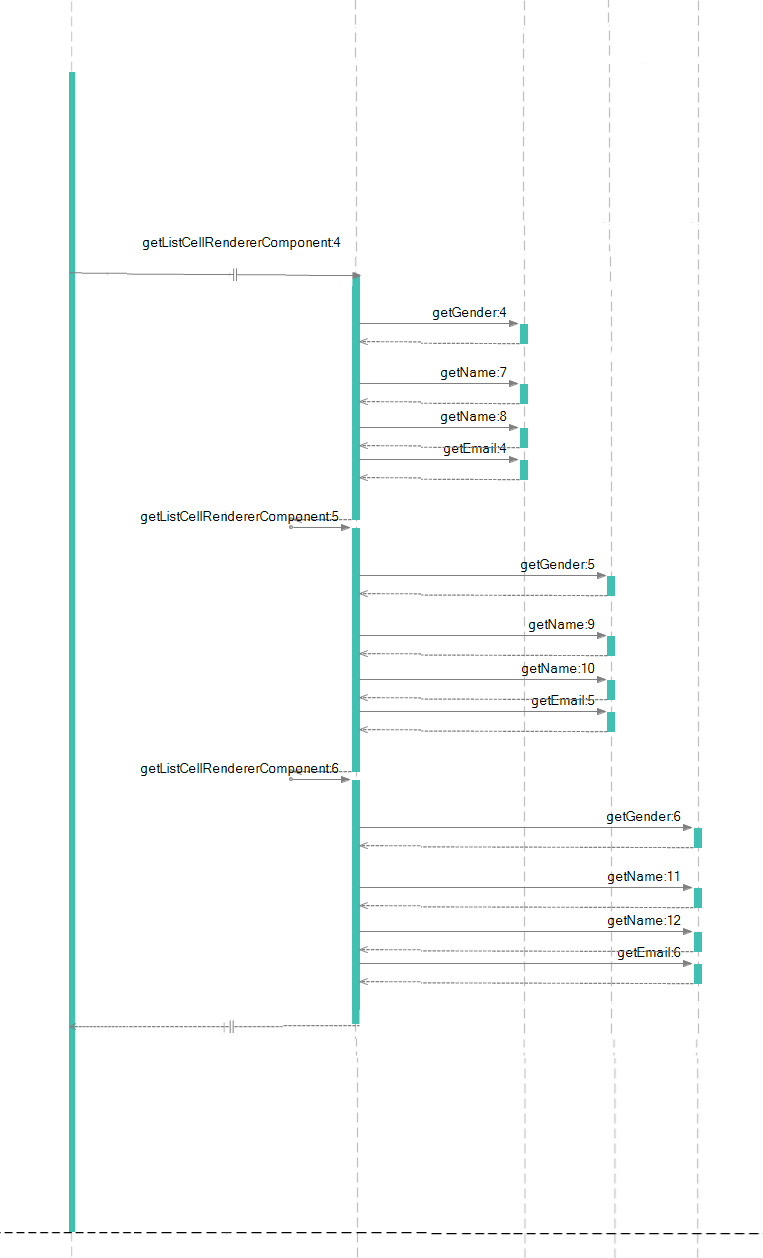
\includegraphics[height =.5\paperheight, trim= 0cm 5cm 0cm 5cm, clip]{MMI-Oving4-SequenceDiagInit-isolatedEventsMock}
	\caption{An example of how \autoref{fig:seqOving4CrossLines} might look in the isolated view}
	\label{fig:seqOving4IsolatedMock}
\end{figure}
~\\

%auto-avspilling av states
Stepping through the recorded states is, as mentioned above, a time-consuming and impractical.
While there are quick and easy ways to jump straight to any interesting state, it may also be interesting to view a playback of a part of, or the entire execution.
This would allow an easier way of observing changes happening in a program.
The playback would automatically step through the recorded states at a pace that the user should be able to adjust, updating the diagrams for each step.
Playback should be possible to initialize from any selected event that has been recorded, as starting from the beginning would often be a waste of time.
~\\

%søk
Searching can be improved by relaxing the requirements for for search-terms.
The requirement of full class names in searches goes against the expected behavior set by both web- and desktop-based search engines, and is likely to cause confusion or, at worst, leave users thinking the functionality is broken.
Relaxing this requirement to allowing partial class names, or substrings in general, would be an improvement to the usability of the tool.
~\\